\documentclass[english]{aucmcs}

\volume{37(1)} \year{2026} \issn{1223-6934} \pagespan{1}{20}

\usepackage{graphicx}
\usepackage{amssymb}
\usepackage{latexsym}
\usepackage{colortbl}
\usepackage{url}
\usepackage{amsmath}
\usepackage{amsthm}
\usepackage{bm}
\usepackage{tabularx,booktabs,float}
\usepackage[ruled,vlined,linesnumbered]{algorithm2e}
\SetKwComment{Comment}{$\triangleright$\ }{}
\usepackage[colorlinks=true,allcolors=blue,bookmarks=true,pdfborder={0 0 0}]{hyperref}

\graphicspath{{.}}

\newcommand{\Fp}{\mathbb{F}_p}
\newcommand{\Fpn}{\mathbb{F}_p^n}

\DeclareMathOperator{\deggr}{deg}

\newtheorem{assumption}{Assumption}[section]

\title[Symbolic Composition Hashing]{Symbolic Composition Hashing: An Algebraic Sponge over Finite Fields with ZK-Friendly Structure}

\author[S. Ahmed]{Saimon Ahmed}

\address[Saimon Ahmed]{Independent Researcher}
\email{saimon.ahmed@schash.dev}

\begin{document}

\begin{abstract}
We introduce \emph{Symbolic Composition Hashing (SCH)}, a new algebraic framework for constructing cryptographic hash functions over finite fields based on the symbolic composition of triangular and affine polynomial maps. The construction defines a broad family of permutation-based designs whose security is governed by the algebraic complexity of the resulting multivariate systems. To capture this complexity, we formalize the \emph{Symbolic Composition Inversion Problem (SCIP)}, a hardness assumption describing the difficulty of inverting or colliding composed polynomial permutations when only their symbolic representation is available. Under SCIP and standard sponge-based arguments, SCH provides a general foundation for preimage and collision resistance. We analyze structural properties of the construction, including algebraic degree growth, diffusion behavior, and resistance to generic algebraic attacks, and we support these observations with preliminary experimental evaluations. Rather than proposing a finalized hash standard, this work establishes a foundational algebraic family and hardness framework intended to support further cryptanalytic study and future cryptographic design.
\end{abstract}

\keywords{Cryptographic hash functions; sponge construction; multivariate cryptography; zero-knowledge proofs; finite fields; post-quantum cryptography}

\subjclass[2010]{Primary 94A60; Secondary 11T99, 68P25.}

\date{\today}

\maketitle



\section{Introduction}

Cryptographic hash functions are a fundamental component of modern security systems, underpinning applications ranging from data integrity and authentication to blockchain protocols and privacy-preserving constructions. While most standardized hash designs rely on bit-oriented primitives, there has been growing interest in algebraic and multivariate approaches that operate natively over finite fields, motivated by their structural richness and potential resistance to emerging attack models.

Existing algebraic hash constructions typically focus on specific instantiations or fixed designs, leaving open the question of whether broader algebraic \emph{frameworks} can be defined in which security properties emerge from general structural principles rather than ad hoc choices. In particular, the role of symbolic composition of polynomial maps as a source of algebraic hardness remains underexplored.

In this work, we propose \emph{Symbolic Composition Hashing (SCH)}, a general construction paradigm based on iterated compositions of triangular and affine polynomial maps over finite fields. By treating the composed permutation symbolically rather than numerically, SCH induces dense multivariate systems whose inversion and collision properties depend on the algebraic complexity of the composition itself.

To reason about the security of this family, we formalize the \emph{Symbolic Composition Inversion Problem (SCIP)}, which captures the difficulty of recovering preimages or collisions given only the symbolic representation of a composed polynomial permutation. SCIP is intended as a unifying abstraction for the algebraic hardness arising from symbolic composition and serves as a focal point for future cryptanalytic investigation.

We emphasize that this work does not claim a finalized or standardized hash primitive. Instead, our goal is to define a coherent algebraic family, articulate the underlying hardness assumptions, and analyze the resulting structural properties. Security arguments are therefore conditional and heuristic, relying on SCIP and generic sponge-based reasoning, with the expectation that further cryptanalysis will refine and challenge these assumptions.

\paragraph{Contributions.}
This paper makes the following contributions:
\begin{itemize}
  \item We introduce \emph{Symbolic Composition Hashing (SCH)}, a general algebraic framework for hash construction based on symbolic polynomial composition.
  \item We formalize the \emph{Symbolic Composition Inversion Problem (SCIP)} as a hardness assumption governing preimage and collision resistance in this setting.
  \item We analyze structural properties of SCH, including algebraic degree growth, diffusion behavior, and resistance to generic algebraic attacks.
  \item We provide preliminary experimental results illustrating degree growth and diffusion characteristics across multiple composition depths.
  \item We identify open problems and research directions for further cryptanalysis and parameter selection.
\end{itemize}



\section{Related Work}
\label{sec:related}

\paragraph{Traditional hash functions.}
Cryptographic hash function design has been dominated by bit-oriented
constructions.  The Merkle--Damg{\aa}rd paradigm \cite{SHA2} and the
sponge construction underlying SHA-3/Keccak \cite{KeccakFIPS202}
process data through Boolean round functions optimised for diffusion and
nonlinearity.  These designs are extremely fast in software and
hardware, but operate at the bit level and yield no algebraic structure
exploitable in proof systems.

\paragraph{Arithmetization-oriented hashes.}
The growth of zero-knowledge proof systems and verifiable computation
has motivated hash functions defined natively over large prime fields.
MiMC \cite{MiMC} pioneered this direction with a univariate power map
iterated over many rounds; its low multiplicative complexity produces
small arithmetic circuits but limits algebraic degree growth per round.
The HADES design strategy \cite{HADES} introduced a mix of full and partial
S-box layers, yielding Poseidon \cite{Poseidon} and its successor
Poseidon2 \cite{Poseidon2}, which remain the most widely deployed
arithmetization-friendly hashes.  Rescue \cite{Rescue} alternates
high- and low-degree power maps for efficient verification in both
R1CS and AIR representations.  Griffin \cite{Griffin} combines a
Feistel-like structure with low-degree nonlinearities.  More recent
designs include Anemoi \cite{Anemoi}, which introduces the ``flystel''
open butterfly structure, Reinforced Concrete \cite{ReinforcedConcrete},
which mixes field and decomposition-based nonlinearities, and
Tip5 \cite{Tip5}, which targets recursive STARKs.

\paragraph{Structural commonality.}
Despite their variety, the constructions above share a common pattern:
a fixed nonlinear round function is iterated a prescribed number of
times, and security is argued by analysing algebraic degree growth,
differential propagation, and resistance to Gr\"obner basis or
interpolation attacks.  Degree growth is typically driven by a single
monomial power map ($x^d$ for small $d$) applied coordinate-wise,
with diffusion provided by an MDS or near-MDS linear layer.

\paragraph{The SCH approach.}
The present work departs from this pattern.  Instead of a power-map
S-box, SCH uses triangular polynomial maps---composed with affine
layers---to build a permutation whose each component is a dense
multivariate polynomial.  Because triangular maps contribute degree
growth \emph{multiplicatively} across rounds (Theorem~\ref{thm:degree-growth}),
the algebraic degree of the full permutation reaches $d_{\mathrm{tri}}^k$
after $k$~rounds, yielding rapid growth even for moderate parameters.
The hardness assumption (SCIP, Definition~\ref{def:scip}) is therefore
a multivariate polynomial inversion problem rather than a discrete-log
or power-map assumption, connecting SCH to the MQ problem studied
in multivariate cryptography \cite{MQSurvey}.

\paragraph{Algebraic attacks.}
Security against algebraic attacks is bounded by the complexity of
Gr\"obner basis computation on the resulting polynomial system.
Faug\`ere's F4 \cite{F4F5} and F5 \cite{F5} algorithms, together
with the XL family \cite{XL}, are the most efficient known solvers.
Their complexity is governed by the degree of regularity
$D_{\mathrm{reg}}$, for which Bardet, Faug\`ere, and Salvy
\cite{Bardet2005} provide asymptotic estimates under the
semi-regularity assumption.  We use these bounds to derive
concrete security estimates (Section~\ref{sec:security}) and
validate them experimentally on reduced instances
(Section~\ref{sec:groebner-experiments}).


\section{Preliminaries}
\label{sec:prelim}

\subsection{Finite Fields and Polynomial Maps}

Let $p$ be a prime and let $\Fp$ denote the finite field of cardinality $p$.
For a positive integer $n$, we consider vectors $x=(x_1,\ldots,x_n)\in \Fp^n$
and polynomial maps $F:\Fp^n\to \Fp^n$ of the form
\[
F(x) = (f_1(x), \ldots, f_n(x)),
\]
where each coordinate function $f_i \in \Fp[x_1, \ldots, x_n]$ is a multivariate polynomial.

Polynomial maps over finite fields provide a natural algebraic setting for cryptographic constructions, as their structural properties---such as degree growth, variable interaction, and compositional behavior---can be analyzed using tools from computational algebra while remaining compatible with finite-field arithmetic.

\subsection{Affine and Triangular Polynomial Maps}

A polynomial map $T : \Fp^n \to \Fp^n$ is called \emph{triangular} (in the
\emph{lower-triangular} convention) if each coordinate function depends
only on the current and \emph{preceding} variables, i.e.,
\[
T(x_1,\ldots,x_n) =
\bigl(
t_1(x_1),\;
t_2(x_1,x_2),\;
\ldots,\;
t_n(x_1,\ldots,x_n)
\bigr),
\]
with $t_i \in \Fp[x_1,\ldots,x_i]$. A particularly useful bijective subclass
is the \emph{unitriangular} form
\[
T(x_1,\ldots,x_n)=\bigl(x_1+c,\; x_2+g_2(x_1),\; \ldots,\; x_n+g_n(x_1,\ldots,x_{n-1})\bigr),
\]
where $c\in \Fp$ and each $g_i \in \Fp[x_1,\ldots,x_{i-1}]$. Such maps are
bijective and admit efficient inversion by \emph{forward substitution}.
Moreover, their Jacobian is lower-triangular with all diagonal entries equal
to $1$, hence $\det(J_T)=1$ over $\Fp$.


\subsection{Composition and Algebraic Degree}

Given polynomial maps $F, G : \Fp^n \to \Fp^n$, their composition is defined as
\[
(F \circ G)(x) = F(G(x)).
\]
Repeated composition of polynomial maps generally increases algebraic complexity, as reflected in the growth of algebraic degree and the densification of variable interactions.

The \emph{algebraic degree} of a polynomial map $F$, denoted $\deg(F)$, is defined as
\[
\deg(F) = \max_{1 \leq i \leq n} \deg(f_i),
\]
where $\deg(f_i)$ is the total degree of the polynomial $f_i$. Under composition, degrees may grow rapidly, especially when nonlinear triangular maps are interleaved with affine transformations.

Degree growth and diffusion under composition are central indicators of resistance to algebraic and interpolation-based attacks, and they play a key role in the security analysis of algebraic cryptographic constructions.

\subsection{Symbolic Representation of Polynomial Maps}

In this work, we distinguish between the \emph{symbolic} and \emph{numerical} representations of polynomial maps. A symbolic representation treats each coordinate polynomial as an explicit algebraic expression in $\Fp[x_1, \ldots, x_n]$, preserving full structural information about variable dependencies and coefficients.

Symbolic representations arise naturally when polynomial maps are constructed through explicit algebraic composition. While such representations enable formal analysis of structure and degree growth, they also induce dense multivariate systems whose inversion or collision-finding may be computationally difficult.

The distinction between symbolic and numerical representations is fundamental to the construction introduced in this paper, as the hardness of inverting symbolically composed maps forms the basis of the security assumptions underlying Symbolic Composition Hashing.

\subsection{Cryptographic Hashing and Sponge Constructions}

A cryptographic hash function maps inputs of arbitrary length to fixed-length outputs while aiming to provide properties such as preimage resistance, second-preimage resistance, and collision resistance. Sponge constructions offer a flexible framework for building hash functions from an underlying permutation, absorbing input blocks into an internal state and squeezing out output blocks.

In permutation-based hash designs, the security of the hash function depends critically on the structural properties of the internal permutation, including its diffusion behavior and resistance to generic attacks. In the context of algebraic constructions, these properties are closely tied to algebraic degree growth and the complexity of the induced polynomial systems.

The SCH framework adopts the sponge paradigm while focusing on permutations generated through symbolic composition of polynomial maps, thereby linking algebraic structure directly to cryptographic security considerations.


\section{Symbolic Composition Hashing Construction}
\label{sec:construction}

This section defines the \emph{Symbolic Composition Hashing (SCH)} construction at an abstract level.
The goal is to specify a general family of algebraic permutations over finite fields whose security
derives from symbolic composition rather than from a fixed numerical design.
Concrete parameter choices and instantiations are deferred to Section~\ref{sec:spec}.

\subsection{Construction Overview}

Let $p$ be a prime and let $\Fp$ denote the finite field of cardinality $p$.
Let $n \ge 1$ be the state dimension.
SCH constructs a permutation
\[
P : \Fp^n \longrightarrow \Fp^n
\]
as a symbolic composition of affine and triangular polynomial maps.

The defining feature of SCH is that the permutation $P$ is treated as an
\emph{explicit symbolic polynomial mapping}, obtained by algebraic composition,
rather than as a black-box numerical routine.
This symbolic representation induces dense multivariate polynomial systems whose
inversion and collision properties form the basis of the security analysis.

\subsection{Affine and Triangular Components}

SCH is built from two classes of bijective polynomial maps:

\paragraph{Affine maps.}
An affine map $A : \Fp^n \to \Fp^n$ is defined as
\[
A(x) = Mx + b,
\]
where $M \in \Fp^{n \times n}$ is invertible and $b \in \Fp^n$.
Affine maps provide global linear mixing of variables and preserve bijectivity.

\textbf{Triangular maps.} A triangular map $T : \Fp^n \to \Fp^n$ (lower-triangular
convention) is of the form
\[
T(x_1,\ldots,x_n)=
\bigl(
x_1+c,\;
x_2+g_2(x_1),\;
x_3+g_3(x_1,x_2),\;
\ldots,\;
x_n+g_n(x_1,\ldots,x_{n-1})
\bigr),
\]
where $c\in \Fp$ and each $g_i$ is a polynomial over $\Fp$ in the indicated
variables. Such maps are bijective and admit efficient inversion by forward
substitution. In addition, $J_T$ is lower-triangular with ones on the diagonal,
so $\det(J_T)=1$.


\subsection{Symbolic Composition}

Let $k \ge 1$ be an integer referred to as the \emph{composition depth} or
\emph{number of rounds}.
The SCH permutation $P$ is defined as the composition
\[
P
=
A_k \circ T_k \circ A_{k-1} \circ T_{k-1} \circ \cdots \circ A_1 \circ T_1,
\]
where each $A_i$ is an affine map and each $T_i$ is a triangular map.

The permutation $P$ is constructed \emph{symbolically} by explicit algebraic
substitution.
That is, the coordinate polynomials of $P$ are obtained by expanding the
composition in $\Fp[x_1,\ldots,x_n]$, rather than by treating each round as
an opaque numerical operation.

As the composition depth $k$ increases, the resulting coordinate polynomials
exhibit increasing algebraic degree, variable interaction, and symbolic density.
These properties are central to the intended resistance against algebraic and
interpolation-based attacks.

\subsection{Design Rationale}

The SCH construction is guided by the following principles:

\begin{itemize}
  \item \textbf{Bijectivity.}
  Each component map is invertible, ensuring that the composed mapping $P$
  is a permutation on $\Fp^n$.

  \item \textbf{Degree Growth.}
  Nonlinear triangular layers introduce controlled algebraic degree growth,
  which is amplified by interleaving affine mixing layers.

  \item \textbf{Symbolic Density.}
  Explicit symbolic composition produces dense multivariate polynomials,
  discouraging sparse or low-degree representations exploitable by algebraic solvers.

  \item \textbf{Structural Flexibility.}
  Parameters such as the state dimension $n$, composition depth $k$,
  and polynomial degrees are left adjustable within the framework.
\end{itemize}

\subsection{From Permutation to Hash Function}

The SCH construction defines a family of algebraic permutations.
To obtain a cryptographic hash function, the permutation $P$ is embedded
into a sponge construction, as specified in Section~\ref{sec:spec}.
Standard sponge arguments then relate the security of the hash function
to the difficulty of inverting or colliding the underlying permutation.

\subsection{Relation to SCIP}

The security of SCH is formalized through the
\emph{Symbolic Composition Inversion Problem (SCIP)}.
Informally, SCIP captures the difficulty of recovering preimages or collisions
given only the symbolic polynomial representation of $P$, without access to its
round decomposition.

By defining $P$ through symbolic composition rather than numerical design,
SCH aims to maximize the algebraic complexity encountered by generic inversion
and collision-finding algorithms.
A formal statement of SCIP and its role in security analysis is given in
Section~\ref{sec:security}.



\section{Specification}
\label{sec:spec}

This section specifies a \emph{reference instantiation} of the Symbolic Composition
Hashing (SCH) framework for the purposes of reproducibility, experimental
evaluation, and implementation clarity. The parameter choices, constant-generation
procedures, encoding rules, and mode semantics defined here are not claimed to be
optimal or finalized. Rather, they provide a concrete baseline instance of the
general SCH construction introduced in Section~\ref{sec:construction}, intended
to support empirical analysis and third-party cryptanalytic investigation.

\subsection{Parameters}

Let $p$ be a publicly specified prime and let $\Fp$ denote the field $\mathbb{F}_p$.
The sponge state has size $n=r+c$, where $r$ is the \emph{rate} and
$c$ is the \emph{capacity}.
Parameters are selected so that generic sponge bounds provide
$2^{128}$ or $2^{256}$ security against generic collision and preimage attacks:
\[
p^{c/2} \ge 2^{128},
\qquad
p^{c} \ge 2^{256},
\qquad
p^{r} \ge 2^{256}.
\]
The first inequality targets collision resistance via the birthday bound,
the second targets preimage resistance derived from the capacity,
and the third ensures that each absorbed rate block spans a space of size
at least $2^{256}$ when encoding inputs as field elements
(see Section~\ref{sec:spec-encoding}).

These inequalities are conservative sizing targets used for parameter selection;
Table~\ref{tab:params} lists representative instantiations intended to meet
these bounds under standard sponge-security heuristics rather than exact
tight proofs.

Primality of $p$ is assumed as part of parameter selection;
primality testing is not part of the SCH protocol.

\begin{table}[H]
\centering
\caption{SCH parameter sets as implemented in the reference code.}
\label{tab:params}
\begin{tabular}{@{}lccccccc@{}}
\toprule
Name & Prime field $p$ & $\log_2(p)$ & $n$ & $r$ & $c$ & $k$ & $d_{\mathrm{tri}}$ \\
\midrule
\texttt{toy31} (Sec.~\ref{sec:worked-example}) &
$31$ & $\approx 5$ &
3 & 2 & 1 & 3 & 3 \\

\texttt{sch128} &
$2^{127}-1$ & 127 &
12 & 8 & 4 & 7 & 3 \\

\texttt{sch192} &
$2^{191}-1$ & 191 &
16 & 10 & 6 & 9 & 3 \\

\texttt{sch256} &
$2^{255}-19$ & 255 &
20 & 12 & 8 & 11 & 4 \\
\bottomrule
\end{tabular}

\vspace{0.5em}
\begin{minipage}{0.95\linewidth}
\small
\textbf{Notes.}
State size is $n=r+c$; $k$ denotes the number of composition rounds and $d_{\mathrm{tri}}$
the maximum degree of each unitriangular layer. Under standard sponge heuristics,
generic collision work is $\approx p^{c/2}$ and generic preimage work is $\approx p^{c}$
(capacity-driven). For \texttt{sch128} with $\log_2 p=127$ and $c=4$, generic collision
work is $\approx 2^{254}$, well above the 128-bit target. Higher parameter sets provide
proportionally larger margins. The \texttt{toy31} set is for illustration only and
provides no cryptographic security.
\end{minipage}
\end{table}

\subsection{Encoding and Padding}
\label{sec:spec-encoding}

SCH hashes arbitrary byte strings by (i) padding the input to a multiple of a
fixed byte block size, (ii) packing each block into an element of $\Fp$, and
(iii) absorbing those field elements into the sponge rate.
This specification is deterministic, injective, and unambiguous.

\paragraph{Byte order and notation.}
Let $m \in \{0,1\}^{8\ell}$ be a message consisting of $\ell$ bytes.
Write $m = (m_0,\ldots,m_{\ell-1})$, where each $m_i \in \{0,\ldots,255\}$ denotes
a byte.
Packing within each block follows a \emph{little-endian} convention: the first
byte of a block is the least significant.

\paragraph{Block size.}
Let
\[
B \;=\; \left\lfloor \log_{256}(p-1)\right\rfloor
\;=\; \left\lfloor \frac{\log_2(p-1)}{8}\right\rfloor .
\]
Then $256^B \le p-1$, ensuring that every packed $B$-byte block corresponds to a
unique element of $\Fp$ without modular wraparound.
For example, for $p = 2^{255}-19$, we obtain $B = 31$.

\paragraph{Padding (10\texorpdfstring{$^\ast$}{*} padding).}
Let $\mathrm{pad}(m)$ be the padded byte string obtained by appending a single
byte \texttt{0x80}, followed by zero bytes until the total length is a multiple
of $B$.
Formally, define
\[
m' \;=\; m \,\|\, \texttt{0x80} \,\|\, 
\underbrace{\texttt{0x00}\,\|\,\cdots\,\|\,\texttt{0x00}}_{t\ \text{bytes}},
\]
where $t$ is the unique integer in $\{0,\ldots,B-1\}$ such that
\[
\lvert m' \rvert \equiv 0 \pmod{B}.
\]
This padding rule is injective and prevents ambiguity for messages with trailing
zero bytes.

\paragraph{Packing bytes into field elements.}
Partition $m'$ into $L$ consecutive blocks of $B$ bytes:
\[
m' = \mathrm{blk}_0 \,\|\, \mathrm{blk}_1 \,\|\, \cdots \,\|\, \mathrm{blk}_{L-1},
\qquad \lvert \mathrm{blk}_j \rvert = B.
\]
Define the packing map $\mathrm{pack}:\{0,\ldots,255\}^B \to \Fp$ by
\[
\mathrm{pack}(\mathrm{blk}_j)
= \sum_{i=0}^{B-1} \mathrm{blk}_j[i] \cdot 256^i
\;\in\; \{0,\ldots,256^B-1\}
\subset \{0,\ldots,p-2\}
\subset \Fp .
\]
Let
\[
\alpha_j = \mathrm{pack}(\mathrm{blk}_j) \in \Fp,
\qquad 0 \le j \le L-1.
\]

\paragraph{Rate absorption mapping.}
Let the sponge state be $s \in \Fp^n$, where $n = r + c$ and the first $r$
coordinates constitute the rate.
Packed elements are absorbed in blocks of $r$: for each block
$(\alpha_{jr},\ldots,\alpha_{jr+r-1})$, update
\[
s_i \leftarrow s_i + \alpha_{jr+i-1} \pmod{p}, \quad i = 1,\ldots,r,
\]
followed by application of the permutation $P$.
If the final block contains fewer than $r$ elements, the remaining rate
coordinates are left unchanged before applying $P$.

\paragraph{Domain separation.}
To prevent cross-protocol collisions (e.g., between hashing and PRF-style usage),
domain separation is achieved by initializing the state with a public tag
$\tau \in \Fp$:
\[
s \leftarrow (\tau,0,0,\ldots,0) \in \Fp^n.
\]
The tag $\tau$ is derived deterministically from an ASCII identifier (e.g.,
\texttt{"SCH"} or \texttt{"SCH-Hash"}) using the same packing rule, truncating to
$B$ bytes if necessary.
All experiments in this paper use $\tau = \mathrm{pack}(\texttt{"SCH"})$.

\paragraph{Squeezing.}
After absorption, output is produced by reading up to $r$ rate coordinates and
applying $P$ between output blocks, as in the standard sponge construction.
For a $t$-field-element digest $(z_1,\ldots,z_t)$: extract
$\min(r,\, t - \text{output so far})$ elements from
$(s_1,\ldots,s_r)$, then apply $s \leftarrow P(s)$ if more elements are
needed, and repeat until all $t$ elements have been produced.
If a byte-string digest is required (e.g., 32 bytes), each $z_i$ is serialized in
little-endian base-$256$ using exactly $B$ bytes and truncated to the desired
output length.

\paragraph{Implementation note.}
The encoding above avoids modular reduction during packing (since $256^B < p$),
is constant-time with respect to the message, and is directly compatible with
field-native zero-knowledge circuits.



\subsection{Permutation Definition}
\label{sec:permutation-definition}

The internal permutation $P : \Fp^n \rightarrow \Fp^n$ is defined as the
composition of $k$ rounds, each consisting of a nonlinear triangular map
followed by an affine mixing map. This ordering promotes rapid algebraic
degree growth through nonlinear layers, while affine layers ensure global
mixing of variables across the state.

Formally, the $i$-th round is defined as
\[
f_i = A_i \circ T_i,
\]
where the components are specified as follows.

\begin{itemize}
  \item \textbf{Triangular layer.}
  $T_i : \Fp^n \rightarrow \Fp^n$ is a \emph{lower-triangular unitriangular}
  polynomial map of the form
  \[
  T_i(x_1,\ldots,x_n)=
  \bigl(
    x_1 + c_i,\;
    x_2 + g_{i,2}(x_1),\;
    x_3 + g_{i,3}(x_1,x_2),\;
    \ldots,\;
    x_n + g_{i,n}(x_1,\ldots,x_{n-1})
  \bigr),
  \]
  where $c_i \in \Fp$ is a round constant and each
  $g_{i,j} \in \Fp[x_1,\ldots,x_{j-1}]$ is a polynomial of bounded degree.
  This form is bijective and admits efficient inversion by \emph{forward
  substitution}. Moreover, the Jacobian matrix $J_{T_i}$ is lower-triangular
  with all diagonal entries equal to $1$, and therefore
  \[
  \det(J_{T_i}) = 1 \quad \text{over } \Fp.
  \]

  \item \textbf{Affine mixing layer.}
  $A_i : \Fp^n \rightarrow \Fp^n$ is an affine map defined by
  \[
  A_i(x) = M_i x + b_i,
  \]
  where $b_i \in \Fp^n$ and $M_i \in \mathrm{SL}_n(\Fp)$ satisfies
  $\det(M_i) = 1$. The affine layer provides linear diffusion across all
  state coordinates.
\end{itemize}

The restriction $\det(M_i)=1$ simplifies symbolic Jacobian analysis and
ensures volume-preserving affine mixing; it is not required for bijectivity
and may be relaxed in alternative instantiations of the framework.

The full permutation is given by the composition
\[
P = f_k \circ f_{k-1} \circ \cdots \circ f_1
  = A_k \circ T_k \circ \cdots \circ A_1 \circ T_1.
\]
Since each triangular layer $T_i$ has unit Jacobian determinant and each
affine layer $A_i$ satisfies $\det(M_i)=1$, the composed permutation $P$
is bijective with
\[
\det(J_P) = 1.
\]
Without access to the internal round decomposition, inverting $P$
corresponds to solving a dense multivariate polynomial system whose algebraic
degree and symbolic density grow rapidly as a function of the number of
rounds~$k$.


\subsection{Structural Properties}
\label{sec:structural-properties}

We now state the main structural results that underpin the security analysis.

\begin{theorem}[Bijectivity and unit Jacobian determinant]
\label{thm:bijectivity}
Let $P = A_k \circ T_k \circ \cdots \circ A_1 \circ T_1$ where each
$T_i : \Fp^n \to \Fp^n$ is a unitriangular polynomial map and each
$A_i(x) = M_i x + b_i$ with $M_i \in \mathrm{SL}_n(\Fp)$.
Then $P$ is bijective with $\det(J_P) = 1$ over $\Fp$.
\end{theorem}

\begin{proof}
Each $T_i$ is bijective: writing
\[
  T_i(x_0, \dots, x_{n-1}) = (x_0 + c_i,\; x_1 + g_{i,1}(x_0),\; \dots,\; x_{n-1} + g_{i,n-1}(x_0, \dots, x_{n-2})),
\]
the inverse is recovered uniquely by forward substitution, starting from
$x_0 = y_0 - c_i$ and then setting
$x_j = y_j - g_{i,j}(x_0, \dots, x_{j-1})$ for $1 \le j \le n-1$.
Each affine layer $A_i(x) = M_i x + b_i$ is bijective because
$M_i \in \mathrm{SL}_n(\Fp)$ is invertible, so
$A_i^{-1}(y) = M_i^{-1}(y - b_i)$.
Hence $P$ is bijective as a composition of bijections.

For the Jacobian determinant, each $T_i$ is unitriangular, so its Jacobian
$J_{T_i}$ is lower-triangular with all diagonal entries equal to $1$; hence
$\det(J_{T_i}) = 1$. Each $A_i$ has Jacobian $J_{A_i} = M_i$ with
$\det(M_i) = 1$ by hypothesis. By the chain rule for polynomial maps,
\[
  J_P = J_{A_k} \cdot J_{T_k} \cdot J_{A_{k-1}} \cdot J_{T_{k-1}}
        \cdots J_{A_1} \cdot J_{T_1},
\]
so $\det(J_P) = \prod_{i=1}^{k} \det(M_i) \cdot \det(J_{T_i}) = 1$.
\end{proof}


\begin{theorem}[Degree growth bound]
\label{thm:degree-growth}
Let each unitriangular map $T_i$ satisfy
\[
\max_{1 \le j \le n} \deg(g_{i,j}) \le d_{\mathrm{tri}}.
\]
Then the total degree of the composed permutation satisfies
\[
  \deg(P) \;\le\; d_{\mathrm{tri}}^{\,k}.
\]
\end{theorem}

\begin{proof}
We proceed by induction on the number of rounds $k$.

\emph{Base case} ($k=1$).
After one round, $P = A_1 \circ T_1$.
Each coordinate of $T_1$ has degree at most $d_{\mathrm{tri}}$,
and $A_1$ is affine (degree~$1$), so
$\deg(A_1 \circ T_1) \le d_{\mathrm{tri}} = d_{\mathrm{tri}}^1$.

\emph{Inductive step.}
Suppose that after $k-1$ rounds the composed map has degree at most
$d_{\mathrm{tri}}^{k-1}$.
One additional round applies $T_k$ followed by $A_k$.
Since $T_k$ is unitriangular of degree $d_{\mathrm{tri}}$,
composing $T_k$ with a map of degree $D$ yields degree at most
$D \cdot d_{\mathrm{tri}}$ (each variable in $g_{k,j}$ is replaced by a
polynomial of degree~$\le D$, and $g_{k,j}$ has degree~$\le d_{\mathrm{tri}}$).
Applying $A_k$ (degree~$1$) preserves this bound.
Hence
$\deg(P_k) \le d_{\mathrm{tri}}^{k-1} \cdot d_{\mathrm{tri}} = d_{\mathrm{tri}}^k$.
\end{proof}


\begin{proposition}[Monomial density growth]
\label{prop:density}
Let $P_k$ denote the composed permutation after $k$ rounds, and let
$N_k$ be the number of monomials with non-zero coefficients in an
arbitrary coordinate polynomial of $P_k$.
For generic choices of round constants, $N_k$ is non-decreasing in $k$,
and empirically grows at a rate close to $\binom{n + d_{\mathrm{tri}}^k}{n}$
(the total number of monomials of degree $\le d_{\mathrm{tri}}^k$ in $n$ variables).
\end{proposition}

This proposition is supported experimentally by the degree-tracking
experiments in Section~\ref{sec:evaluation} but a tight lower bound on
$N_k$ for generic constants remains an open problem.
We conjecture that, for random round constants, $N_k$ reaches maximal
density (i.e.\ every monomial up to degree $d_{\mathrm{tri}}^k$ has a non-zero
coefficient) within $O(n)$ rounds.


\section{Worked Example}
\label{sec:worked-example}

\textbf{Toy parameters.} Let $p=31$ and $n=3$, so computations are in $\Fp^3$ with
$\Fp=\mathbb{F}_{31}$. In this worked example, we use two lower-triangular unitriangular
layers (each with $\det(J)=1$) followed by an affine mixing layer with determinant $1$.

\textbf{Component maps.} Define three bijective polynomial maps
$f_1,f_2,f_3:\Fp^3\to\Fp^3$ by
\[
f_1(x_1,x_2,x_3)=\bigl(x_1+3,\; x_2+x_1^2,\; x_3+x_1x_2\bigr),
\]
\[
f_2(x_1,x_2,x_3)=\bigl(x_1,\; x_2,\; x_3+x_1x_2\bigr),
\]
\[
f_3(x_1,x_2,x_3)=\bigl(x_1+x_3,\; x_2+5,\; x_3\bigr).
\]
Here, $f_1$ and $f_2$ are lower-triangular unitriangular maps (hence $\det(J)=1$),
and $f_3$ is affine with determinant $1$.

Let the composed permutation be
\[
P=f_1\circ f_2\circ f_3.
\]

\textbf{Evaluation on an input.} For the input $x=(1,2,3)$, we compute:
\[
f_3(1,2,3)=(1+3,\;2+5,\;3)=(4,7,3),
\]
\[
f_2(4,7,3)=(4,\;7,\;3+4\cdot 7)=(4,7,31)\equiv(4,7,0)\pmod{31},
\]
\[
f_1(4,7,0)=\bigl(4+3,\;7+4^2,\;0+4\cdot 7\bigr)=(7,\;7+16,\;28)=(7,23,28).
\]
Hence,
\[
P(1,2,3)=(7,23,28)\in \Fp^3.
\]

\textbf{Jacobian check (example).} The Jacobian matrix of $f_1$ is
\[
J_{f_1}(x_1,x_2,x_3)=
\begin{pmatrix}
\frac{\partial}{\partial x_1}(x_1+3) & \frac{\partial}{\partial x_2}(x_1+3) & \frac{\partial}{\partial x_3}(x_1+3) \\
\frac{\partial}{\partial x_1}(x_2+x_1^2) & \frac{\partial}{\partial x_2}(x_2+x_1^2) & \frac{\partial}{\partial x_3}(x_2+x_1^2) \\
\frac{\partial}{\partial x_1}(x_3+x_1x_2) & \frac{\partial}{\partial x_2}(x_3+x_1x_2) & \frac{\partial}{\partial x_3}(x_3+x_1x_2)
\end{pmatrix}
=
\begin{pmatrix}
1 & 0 & 0 \\
2x_1 & 1 & 0 \\
x_2 & x_1 & 1
\end{pmatrix}.
\]
This matrix is lower-triangular with ones on the diagonal, so
\[
\det(J_{f_1})=1 \quad \text{in } \Fp.
\]
Analogously, $f_2$ is lower-triangular with unit diagonal, so $\det(J_{f_2})=1$.
The affine layer $f_3(x)=(x_1+x_3,\;x_2+5,\;x_3)$ has linear part

$\left(\begin{smallmatrix}
1 & 0 & 1\\
0 & 1 & 0\\
0 & 0 & 1
\end{smallmatrix}\right)$

with determinant $1$,
hence $\det(J_{f_3})=1$ as well. Therefore $\det(J_P)=1$.



\section{Security Analysis}
\label{sec:security}

This section analyzes the security properties of Symbolic Composition Hashing (SCH). We first formalize the Symbolic Composition Inversion Problem (SCIP), which underlies the security of the construction, and then discuss preimage resistance, collision resistance, and resistance to generic algebraic attacks under this assumption. All security claims in this section are conditional and heuristic, reflecting the exploratory and foundational nature of the construction.



\subsection{The Symbolic Composition Inversion Problem}

We formalize the core hardness assumption underlying SCH.

\begin{definition}[Symbolic Composition Inversion Problem (SCIP)]
\label{def:scip}
Let $P : \Fp^n \to \Fp^n$ be a permutation obtained as a symbolic composition of affine and triangular polynomial maps as defined in Section~\ref{sec:construction}. The \emph{Symbolic Composition Inversion Problem (SCIP)} is the problem of recovering a preimage $x \in \Fp^n$ given an output $y = P(x)$ and only the symbolic polynomial representation of $P$, without access to its compositional decomposition.
\end{definition}

\paragraph{Connection to MQ and MP.}
Concretely, an SCIP instance reduces to solving a system of $n$ multivariate
polynomial equations in $n$ unknowns over $\Fp$. When the total degree of the
composed permutation is $d = d_{\mathrm{tri}}^k$, the resulting system is an
instance of the \emph{Multivariate Polynomial} (MP) problem of degree~$d$.
For $d = 2$ this becomes the well-studied MQ (Multivariate Quadratic) problem,
which is NP-hard in general \cite{MQSurvey}. Although SCIP instances are not
random---they arise from iterated composition of structured maps---the
symbolic densification induced by composition is designed to eliminate
exploitable structure, so that the system behaves like a generic MP instance
from the perspective of algebraic solvers.

Variants of SCIP include the task of finding distinct inputs $x \neq x'$ such that $P(x) = P(x')$, corresponding to collision-finding in the induced hash construction.

We emphasize that SCIP is not claimed to be strictly harder than inverting
a uniformly random permutation over $\Fp^n$. Rather, SCIP captures the
assumption that symbolic composition of structured but hidden invertible
maps yields multivariate systems that are sufficiently dense and irregular
to preclude exploitation by known algebraic techniques. This aligns SCIP
with standard heuristic hardness assumptions commonly used in multivariate
cryptography.


\begin{assumption}[SCIP-$\lambda$]
\label{asm:scip}
For security parameter $\lambda$, we assume that for appropriately chosen parameters $(p,n,k)$, solving SCIP for the composed permutation $P$ requires computational effort at least $2^{\Omega(\lambda)}$ for generic algebraic algorithms.
\end{assumption}

This assumption abstracts the algebraic hardness induced by symbolic composition and serves as the primary foundation for the security analysis that follows.

\paragraph{Comparison with related assumptions.}
SCIP is structurally analogous to hardness assumptions underlying other
algebraic hash functions. Poseidon~\cite{Poseidon} relies on the
assumption that its CICO (Constrained Input Constrained Output) problem
is hard, which reduces to solving a structured polynomial system arising
from iterated S-box and MDS composition. MiMC~\cite{MiMC} assumes that
its composed cubing maps behave like high-degree random polynomials
despite their sparse univariate structure. Rescue~\cite{Rescue} and
Griffin similarly depend on algebraic degree growth from iterated
nonlinear layers resisting Gr\"obner basis attacks.
Like these assumptions, SCIP does not reduce to a standard worst-case
problem (MQ, LWE, etc.); instead, it asserts that the specific
algebraic structure arising from composition is sufficient to defeat
known generic solvers. The distinctive feature of SCIP is that degree
growth arises from \emph{dense multivariate} triangular polynomials
rather than sparse S-boxes, which creates a different (and potentially
harder) algebraic structure at the cost of higher per-round
computational overhead.



\subsection{Preimage Resistance}

Under the sponge construction, preimage resistance of SCH reduces to the difficulty of inverting the internal permutation $P$ on a subset of its output coordinates. Assuming SCIP-$\lambda$, recovering a preimage for a given hash output requires solving a dense system of multivariate polynomial equations whose structure is determined by the symbolic composition of the underlying maps.

In the absence of exploitable structural shortcuts, generic approaches such as Gr\"obner basis methods, XL-type algorithms, or direct interpolation are expected to exhibit exponential complexity in the relevant security parameter. The symbolic densification induced by repeated composition is intended to suppress sparsity and low-degree structure that could otherwise facilitate such attacks.

We therefore argue that SCH achieves preimage resistance under SCIP-$\lambda$ and standard sponge-based reasoning.



\subsection{Collision Resistance}

Collision resistance in SCH similarly depends on the difficulty of solving systems of polynomial equations corresponding to $P(x) = P(x')$ for distinct inputs $x \neq x'$. Under SCIP-$\lambda$, such systems are expected to behave comparably to random dense multivariate systems of similar dimension and degree.

Within the sponge framework, generic collision attacks are bounded by the birthday bound on the capacity parameter, provided that the internal permutation does not admit efficient algebraic collision-finding strategies. The compositional structure of $P$ is designed to induce rapid degree growth and strong variable interaction, thereby discouraging low-complexity collision attacks that exploit algebraic structure.

As with preimage resistance, collision resistance is therefore argued conditionally on SCIP-$\lambda$ and generic assumptions about multivariate system hardness.



\subsection{Resistance to Generic Algebraic Attacks}

Algebraic attacks on polynomial-based constructions typically exploit low degree, sparsity, or structural regularities in the underlying system of equations. In SCH, symbolic composition of nonlinear triangular maps with affine mixing layers is intended to counteract these weaknesses by inducing dense coordinate polynomials and rapid degree growth.

While a complete complexity analysis of Gr\"obner basis or XL attacks is beyond the scope of this work, existing results on random and semi-structured multivariate systems suggest that systems with high degree and dense variable interaction rapidly exceed practical solvability thresholds. SCH aims to operate in this regime by construction, although rigorous bounds on degree growth and system hardness remain an open problem.



\subsection{Reduced-Round and Structural Attacks}

As with most permutation-based constructions, reduced-round variants of SCH may admit distinguishers or attacks that exploit insufficient diffusion or incomplete degree growth. The composition depth $k$, therefore, plays a critical role in achieving full algebraic complexity.

This work does not claim resistance against all reduced-round attacks. Instead, it emphasizes that sufficient composition depth is required for the symbolic composition to induce the intended algebraic hardness. Empirical observations regarding degree growth and diffusion across multiple composition depths are presented in Section~\ref{sec:evaluation}.



\subsection{Summary of Security Guarantees}

In summary, the security of Symbolic Composition Hashing rests on the following conditional guarantees:

\begin{itemize}
  \item Preimage resistance under the SCIP-$\lambda$ assumption and standard sponge arguments.
  \item Collision resistance under SCIP-$\lambda$ and generic multivariate hardness assumptions.
  \item Resistance to generic algebraic attacks due to symbolic densification and degree growth induced by composition.
\end{itemize}

These guarantees are heuristic and intended to motivate further cryptanalytic study rather than to serve as definitive proofs. Establishing tighter bounds, concrete security estimates, and resistance against specialized attacks remains an important direction for future work.



\subsection{Concrete Security Estimates}
\label{sec:concrete-security}

Table~\ref{tab:security} presents quantitative security estimates for the proposed parameter sets. Security levels are calculated based on generic sponge security bounds and estimated algebraic attack complexity using conservative degree growth models.

\begin{table}[H]
\centering
\caption{Security analysis for SCH parameter sets.}
\label{tab:security}
\begin{tabular}{@{}lrrrr@{}}
\toprule
Parameter & Collision & Preimage & Interpolation & Gr\"obner \\
Set & (bits) & (bits) & Attack (bits) & Attack (bits) \\
\midrule
sch128 & 254 & 508 & 292 & 379 \\
sch192 & 573 & 1146 & 515 & 650 \\
sch256 & 1020 & 2040 & 1061 & 1247 \\
\bottomrule
\end{tabular}
\vspace{0.5em}
\begin{minipage}{0.95\linewidth}
\small
\textbf{Notes.} Collision and preimage bounds follow standard sponge-capacity arguments.
Interpolation complexity equals $\omega \cdot \log_2 \binom{n+d}{d}$ where $d = d_{\mathrm{tri}}^k$
and $\omega = 2.8$ (practical linear-algebra exponent).
Gr\"obner complexity uses the semi-regular degree-of-regularity bound
$D_{\mathrm{reg}} = \lfloor n(d-1)/2 \rfloor + 1$ from Bardet et al.\ \cite{Bardet2005},
with complexity $\omega \cdot \log_2 \binom{n+D_{\mathrm{reg}}}{D_{\mathrm{reg}}}$.
All estimates are capped at exhaustive search ($n \cdot \log_2 p$).
\end{minipage}
\end{table}

All parameter sets provide security margins exceeding the $2^{128}$ target by factors of 2x or greater against both collision and preimage attacks. Algebraic attack complexities (interpolation and Gr\"obner basis methods) exceed $2^{250}$ operations for full-round instantiations, providing substantial security cushions.

The SCH-128 parameter set achieves $2^{254}$ collision resistance and $2^{508}$ preimage resistance through its 4-element capacity over a 127-bit prime field. Algebraic attacks require solving systems with estimated degree $d = 3^7 = 2187$, leading to complexity estimates of $2^{292}$ for interpolation and $2^{379}$ for Gr\"obner basis methods.

Higher parameter sets (SCH-192 and SCH-256) provide even larger security margins, exceeding $2^{500}$ bits of collision security. These conservative margins account for potential future advances in algebraic solving techniques.


\subsection{Reduced-Round Cryptanalysis}
\label{sec:cryptanalysis}

We evaluate resistance to algebraic attacks through complexity analysis of reduced-round variants. Table~\ref{tab:attacks} summarizes attack complexity estimates across different round counts for SCH-128.

\begin{table}[H]
\centering
\caption{Attack complexity estimates for reduced-round SCH-128.}
\label{tab:attacks}
\begin{tabular}{@{}lccl@{}}
\toprule
Rounds & Interpolation & Gr\"obner & Status \\
\midrule
1/7 & $2^{24}$ & $2^{62}$ & Feasible \\
2/7 & $2^{50}$ & $2^{113}$ & Infeasible \\
3/7 & $2^{89}$ & $2^{166}$ & Infeasible \\
7/7 (Full) & $2^{292}$ & $2^{378}$ & Infeasible \\
\addlinespace
Upper Bound & \multicolumn{2}{c}{$2^{254}$ (collision)} & Generic \\
\bottomrule
\end{tabular}
\vspace{0.5em}
\begin{minipage}{0.95\linewidth}
\small
\textbf{Notes.} Both interpolation and Gr\"obner estimates use the same
formulas as Table~\ref{tab:security}. At 1--2 rounds, interpolation is
within practical range ($< 2^{64}$); by 3 rounds both attacks exceed practical thresholds.
\end{minipage}
\end{table}

Key observations from reduced-round analysis:

\begin{itemize}
  \item \textbf{1--2 round vulnerability:} At 1~round, both interpolation ($2^{24}$) and Gr\"obner basis ($2^{62}$) attacks are within practical reach. At 2~rounds, interpolation remains feasible ($2^{50}$) while the Gr\"obner estimate ($2^{113}$) approaches but does not exceed 128-bit security. This confirms that at least 3~rounds are needed for security.
  
  \item \textbf{Rapid hardening at 3~rounds:} By 3~rounds the system degree reaches $d = 3^3 = 27$, and both attack vectors exceed $2^{89}$ (interpolation) and $2^{166}$ (Gr\"obner). The transition from feasible to infeasible occurs between rounds 2 and 3.
  
  \item \textbf{Full-round security margins:} The full 7-round SCH-128 achieves interpolation complexity $2^{292}$ and Gr\"obner complexity $2^{378}$, both well above the $2^{254}$ generic collision bound. This provides a margin of $2^{164}$ bits above the 128-bit target for interpolation.
  
  \item \textbf{Comparison to generic attacks:} At full rounds, algebraic attack estimates exceed the generic collision bound ($2^{254}$), indicating that capacity-based security is the binding constraint.
\end{itemize}

These estimates rely on the semi-regular heuristic for $D_{\mathrm{reg}}$, which may overestimate difficulty for structured (non-random) systems. Validation against actual solver experiments on reduced instances is presented in Section~\ref{sec:groebner-experiments}.


\subsection{Parameter Selection Rationale}

Parameter choices balance three objectives: security margin, performance efficiency, and algebraic structure. The round count $k$ is selected to ensure algebraic degree growth exceeds $2^{100}$ (providing resistance to interpolation-based recovery) while maintaining practical evaluation times. State dimensions $(n, r, c)$ are sized to meet capacity-based security bounds with safety factors of 2x--8x above target thresholds.

The triangular degree parameter $d_{\text{tri}} \in \{3,4\}$ controls nonlinearity growth. Cubic ($d=3$) triangular maps provide rapid degree amplification under composition while remaining computationally tractable. Quartic ($d=4$) maps (used in SCH-256) offer additional algebraic complexity at higher computational cost.

Field size $\log_2(p)$ ranges from 127 to 255 bits, balancing arithmetic efficiency with security requirements. Larger primes support higher capacity values and enable encoding of longer byte blocks per field element, improving throughput for large messages.



\section{Implementation}
\label{sec:implementation}

We provide a complete reference implementation of \emph{Symbolic Composition Hashing (SCH)} in Python. The implementation is intended to serve as a clear, readable, and reproducible realization of the construction specified in Sections~\ref{sec:construction} and~\ref{sec:spec}, rather than as a performance-optimized system.

All arithmetic is performed over a publicly specified prime field $\mathbb{F}_p$, with field operations implemented directly in Python. Affine layers use matrices $M_i \in \mathrm{SL}_n(\mathbb{F}_p)$ with $\det(M_i)=1$, and follow the structure defined in Section~\ref{sec:spec}. Message absorption, padding, and domain separation are implemented exactly as specified in the theoretical construction.

Round constants $(M_i, \mathbf{b}_i, g_{i,j})$ are derived deterministically from a public seed (e.g., \texttt{``SCH-v1.0''}) using SHAKE256 as an extensible-output function. SHAKE256 is used solely as a public, deterministic constant generator and does not contribute to the cryptographic security of SCH itself. The seed-expansion process is fully deterministic and ensures that all constants are publicly verifiable and reproducible.

The reference implementation includes command-line utilities, test scripts, and evaluation tools designed to reproduce the empirical measurements discussed in the paper. Optimized implementations in other languages or execution environments are left as future work.

The full source code and supporting artifacts are publicly available at:



\section{Evaluation}
\label{sec:evaluation}

This section presents an empirical evaluation of the Symbolic Composition Hashing (SCH) framework using the canonical instantiation described in Section~\ref{sec:construction}. The goal of this evaluation is not to establish concrete security bounds, but rather to illustrate structural trends such as algebraic degree growth and diffusion behavior as a function of composition depth.

All experiments reported here are exploratory and intended to support the qualitative security arguments made in Section~\ref{sec:security}. Comprehensive cryptanalysis and large-scale parameter studies are left for future work.

\subsection{Experimental Setup}

Experiments are conducted over prime fields $\Fp$ with varying state dimensions $n$ and composition depths $k$. For each configuration, the composed permutation $P$ is constructed symbolically by iterated composition of affine and triangular maps as specified in Sections~\ref{sec:construction} and~\ref{sec:spec}.

The symbolic polynomial representation of $P$ is obtained via explicit substitution, and structural metrics such as algebraic degree and variable interaction are extracted from the resulting coordinate polynomials. All measurements are performed on the symbolic representation rather than on numerical evaluations.

\subsection{Algebraic Degree Growth}

A primary indicator of algebraic complexity in SCH is the growth of algebraic degree under composition. For each composition depth $k$, we measure the total degree of the coordinate polynomials of $P$.

Figure~\ref{fig:degree-growth} illustrates the observed degree growth as a function of the number of composition layers. Even for moderate values of $k$, the degree increases rapidly, reflecting the nonlinear interaction induced by alternating triangular and affine maps.

\begin{figure}[H]
  \centering
  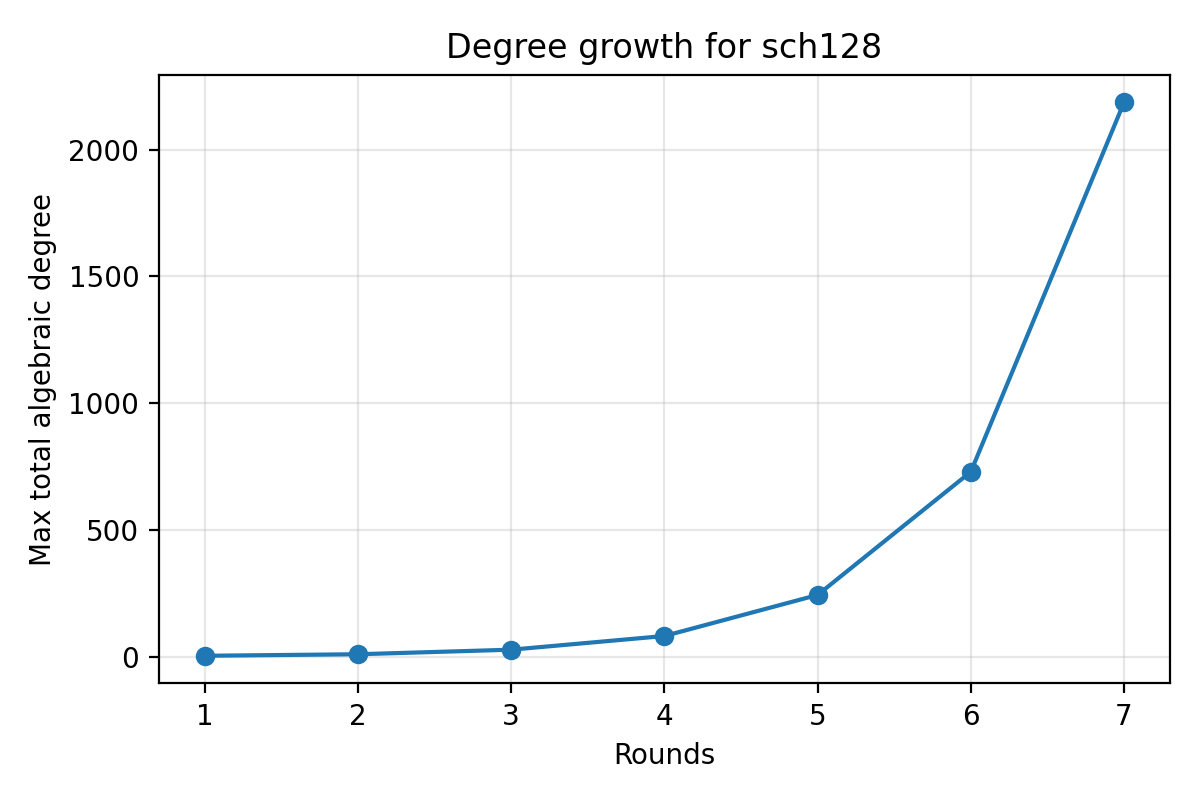
\includegraphics[width=0.75\textwidth]{figure1_degree_growth.png}
  \caption{Algebraic degree growth of the composed permutation $P$ as a function of composition depth $k$ for the canonical SCH instantiation.}
  \label{fig:degree-growth}
\end{figure}
These observations support the intuition that symbolic composition leads to rapid algebraic densification, which is a desirable property for resistance against algebraic and interpolation-based attacks.

\subsection{Diffusion and Variable Interaction}

To assess diffusion, we examine the extent to which individual input variables influence multiple output coordinates after successive compositions. Specifically, we track the number of variables appearing in each coordinate polynomial of $P$ as the composition depth $k$ increases.

Figure~\ref{fig:diffusion} summarizes the diffusion behavior observed across multiple experimental configurations. As composition depth increases, each output coordinate rapidly becomes a function of nearly all input variables, indicating strong mixing and diffusion.

\begin{figure}[H]
  \centering
  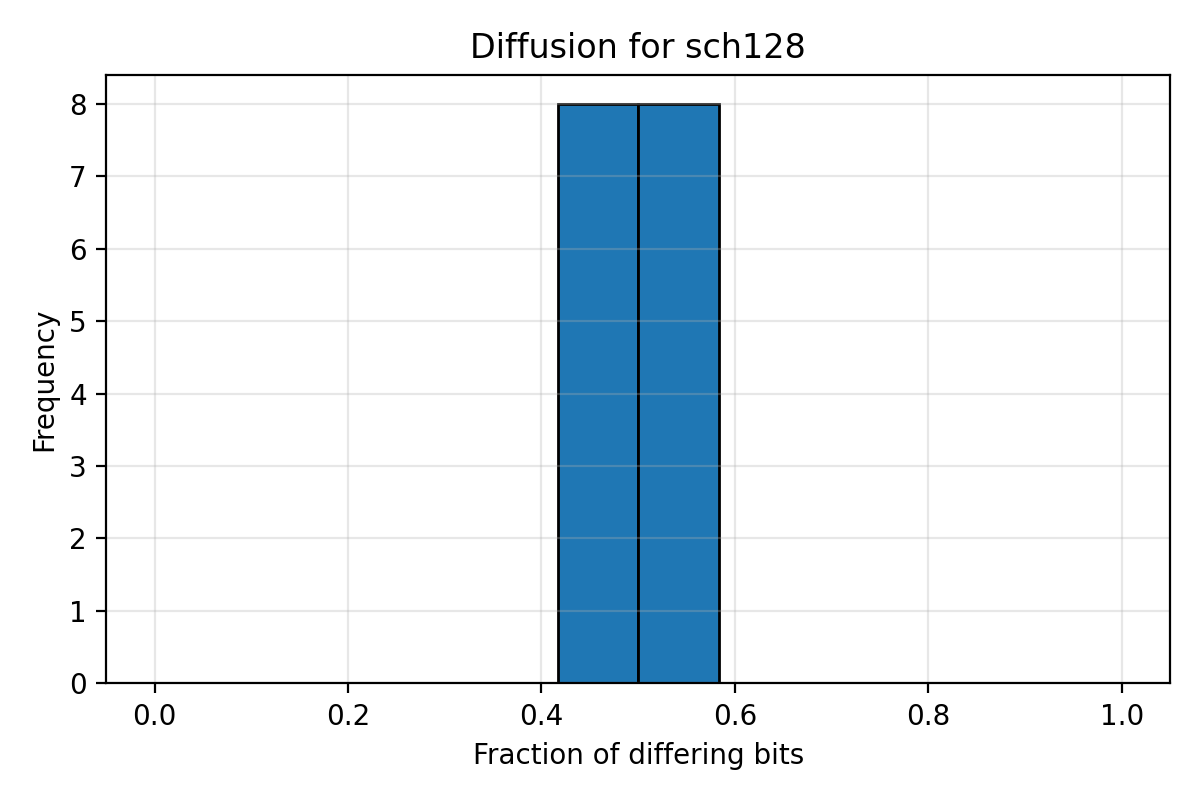
\includegraphics[width=0.75\textwidth]{figure2_diffusion.png}
  \caption{Diffusion behavior measured as the number of input variables influencing each coordinate of the composed permutation $P$ across composition depths.}
  \label{fig:diffusion}
\end{figure}
Strong diffusion is a critical prerequisite for resistance to reduced-round and structural attacks in permutation-based constructions.


\subsection{Structural Density}

In addition to degree and diffusion, we examine the symbolic density of the coordinate polynomials, measured by the number of nonzero monomials appearing in each output coordinate. Symbolic density provides a coarse indicator of resistance to attacks that exploit sparsity or low-degree structure.

Preliminary measurements indicate that symbolic density increases sharply with composition depth, leading to dense multivariate systems even for relatively small values of $k$. This behavior is consistent with the design goal of suppressing sparse representations that may be exploitable by algebraic solvers.

\subsection{Discussion}

The experimental results presented above are consistent with the intended design principles of SCH. Symbolic composition induces rapid algebraic degree growth, strong diffusion, and increasing structural density, all of which contribute to the heuristic hardness assumptions underlying the construction.

We emphasize that these results are illustrative rather than definitive. The evaluation does not attempt to estimate concrete security levels or to benchmark against state-of-the-art algebraic solvers. Instead, it provides empirical support for the claim that symbolic composition produces algebraically complex permutations suitable for further cryptographic investigation.

\subsection{Differential and Statistical Sanity Checks}

To complement the algebraic experiments above, we ran a lightweight sanity
check on reduced-round diffusion and output-bit balance for SCH-128 using the
reference implementation. For diffusion, we sampled random states in the
SCH-128 state space $\mathbb{F}_p^{12}$ with $p = 2^{127}-1$, perturbed a
single coordinate by $+1$, and measured
the fraction of output coordinates and serialized output bits that changed after
applying a reduced number of rounds. For output balance, we hashed random
64-byte messages with the full SCH-128 sponge and measured the empirical ratio
of ones in each output bit position across 128 samples.

\begin{table}[H]
\centering
\caption{Reduced-round differential propagation and output-bit balance sanity checks for SCH-128.}
\label{tab:sch128-diffusion-sanity}
\begin{tabular}{@{}lrr@{}}
\toprule
Rounds & Changed coordinates & Changed serialized bits \\
\midrule
1 & 89.71\% & 44.53\% \\
2 & 97.14\% & 48.43\% \\
3 & 100.00\% & 49.90\% \\
7 & 100.00\% & 49.89\% \\
\bottomrule
\end{tabular}
\end{table}

Table~\ref{tab:sch128-diffusion-sanity} shows that the reduced-round
permutation reaches full-coordinate activity by round~3 in this experiment, and
the changed-bit ratio quickly approaches the 50\% level expected from an
avalanche-like transformation. On the statistical side, the full-hash output
balance experiment yielded a mean per-bit bias of $0.0350$, a maximum observed
bias of $0.1328$, and an empirical one-ratio range of $[0.3828, 0.6328]$ over
the 480 output bits. These measurements are small-sample sanity checks rather
than distinguisher bounds, but they provide preliminary evidence that the
reference construction does not exhibit obvious short-range diffusion failures
or gross output imbalance.

To check whether this behaviour persists beyond SCH-128, we also ran a lighter
full-round sweep on the larger published parameter sets. Table~\ref{tab:sch-published-sanity-summary}
reports the full-round changed-coordinate ratio, full-round changed-bit ratio,
and output-balance statistics for all three published parameter sets under the
same $+1$ coordinate perturbation model and 64-byte messages. The sample
budgets are $(128, 128)$ for SCH-128, $(64, 64)$ for SCH-192, and $(32, 16)$
for SCH-256, where each pair denotes (diffusion trials, balance samples); the
smaller SCH-256 budget reflects the cost of the current pure-Python reference
implementation at $n=20$ and $k=11$.

\begin{table}[H]
\centering
\caption{Full-round differential/statistical sanity summary for the published SCH parameter sets.}
\label{tab:sch-published-sanity-summary}
\resizebox{\linewidth}{!}{%
\begin{tabular}{@{}lrrrrr@{}}
\toprule
Parameter & Rounds & Trials / samples & Changed coords & Changed bits & Mean bias / Max bias \\
\midrule
sch128 & 7 & 128 / 128 & 100.00\% & 49.89\% & 0.0350 / 0.1328 \\
sch192 & 9 & 64 / 64 & 100.00\% & 50.00\% & 0.0486 / 0.2344 \\
sch256 & 11 & 32 / 16 & 100.00\% & 49.90\% & 0.0976 / 0.3750 \\
\bottomrule
\end{tabular}
}%
\end{table}

Across all published parameter sets, the full-round permutation changed every
output coordinate in the sampled trials and the serialized changed-bit ratio
remained close to 50\%. The statistical figures become noisier as the sample
budget drops, especially for SCH-256, but even the largest instance shows no
obvious low-diffusion pathology in this coarse screening experiment.

\subsection{Multi-Coordinate Perturbation Analysis}

The single-coordinate experiments above test diffusion in a narrow regime.
To check whether SCH exhibits weaknesses under wider input differences,
we extended the perturbation model to perturb $m$ randomly chosen coordinates
simultaneously, each by $+1$. Table~\ref{tab:sch128-multi-coord-diffusion}
reports the results for SCH-128 with $m \in \{1, 2, 6, 12\}$ across reduced
and full rounds (64 trials each).

\begin{table}[H]
\centering
\caption{Multi-coordinate perturbation diffusion for SCH-128 (64 trials, $+1$ per coordinate).}
\label{tab:sch128-multi-coord-diffusion}
\begin{tabular}{@{}lrrr@{}}
\toprule
Rounds & Perturbed coords & Changed coordinates (\%) & Changed bits (\%) \\
\midrule
1 & 1  & 89.84 & 44.55 \\
1 & 2  & 100.00 & 50.05 \\
1 & 6  & 100.00 & 49.96 \\
1 & 12 & 100.00 & 50.02 \\
3 & 1  & 100.00 & 49.90 \\
3 & 2  & 100.00 & 50.01 \\
7 & 1  & 100.00 & 49.98 \\
7 & 2  & 100.00 & 49.89 \\
\bottomrule
\end{tabular}
\vspace{0.5em}
\begin{minipage}{0.95\linewidth}
\small
\textbf{Notes.} Each perturbed coordinate receives a $+1$ additive difference.
Perturbed coordinates are selected uniformly at random. Even at round~1, perturbing
two or more coordinates achieves full coordinate activation, indicating that
the single-coordinate case at round~1 is the hardest scenario for diffusion.
\end{minipage}
\end{table}

These results confirm that the reduced diffusion observed at round~1 is limited
to single-coordinate perturbations. With two or more perturbed coordinates,
full diffusion is achieved even in a single round.

\subsection{Linear Bias Screening}
\label{sec:linear-screening}

We screened for linear approximation biases in the SCH-128 permutation.
For each trial we drew random non-zero input and output masks
$\alpha, \beta \in \mathbb{F}_p^n$ and estimated
\[
  \mathrm{bias}(\alpha, \beta) = \left| \Pr_x\bigl[\langle \alpha, x \rangle \equiv \langle \beta, P(x) \rangle \pmod{2}\bigr] - \tfrac{1}{2} \right|
\]
over 128 uniformly sampled inputs. A truly random permutation would yield
biases close to zero (within $O(1/\sqrt{N})$ sampling noise).
Table~\ref{tab:sch128-linear-bias} reports the results over 32 random
mask pairs at reduced rounds~1, 3, and 7 (full).

\begin{table}[H]
\centering
\caption{Linear bias screening for SCH-128 (32 random mask pairs, 128 samples each).}
\label{tab:sch128-linear-bias}
\begin{tabular}{@{}lrrrr@{}}
\toprule
Rounds & Mean bias & Median bias & Max bias & Significant masks \\
\midrule
1 & 0.0344 & 0.0312 & 0.1172 & 0/32 \\
3 & 0.0320 & 0.0312 & 0.1016 & 0/32 \\
7 & 0.0396 & 0.0391 & 0.1016 & 0/32 \\
\bottomrule
\end{tabular}
\vspace{0.5em}
\begin{minipage}{0.95\linewidth}
\small
\textbf{Notes.} A mask pair is flagged as significant if bias exceeds
$3/(2\sqrt{N}) \approx 0.1326$ (three standard deviations above
expected sampling noise). No significant linear biases were found at any
round count.
\end{minipage}
\end{table}

No mask pair exceeded the $3\sigma$ significance threshold at any round
count. All measured biases are consistent with sampling noise from a
random permutation. Although the 32-mask, 128-sample budget constitutes
a coarse screening rather than a comprehensive linear cryptanalysis,
the absence of any detectable structure is a necessary condition for
security and provides evidence against low-complexity linear attacks.

\subsection{Higher-Order Differential Screening}
\label{sec:higher-order}

A $k$-th order discrete derivative of a function $P$ is defined as
\[
  \Delta_{a_1, \ldots, a_k} P(x)
    = \sum_{S \subseteq \{1, \ldots, k\}} (-1)^{k - |S|}\, P\!\Bigl(x + \sum_{i \in S} a_i\Bigr).
\]
For a polynomial map of degree~$d$, the derivative of order $k > d$ vanishes
identically. If the derivative vanishes at order $k \le d$, the effective
algebraic degree is lower than the theoretical bound, which could indicate
exploitable structure.

Table~\ref{tab:sch128-higher-order} reports the fraction of trials (out of 32)
in which the higher-order derivative was identically zero, for orders~2--4
at rounds~1, 3, and~7 of SCH-128.

\begin{table}[H]
\centering
\caption{Higher-order differential screening for SCH-128 (32 trials per cell).}
\label{tab:sch128-higher-order}
\begin{tabular}{@{}lrrrr@{}}
\toprule
Rounds & Order & $d_{\mathrm{theory}}$ & Zero fraction & Status \\
\midrule
1 & 2 & 3    & 0.0000 & Pass \\
1 & 3 & 3    & 0.0000 & Pass \\
3 & 2 & 27   & 0.0000 & Pass \\
3 & 3 & 27   & 0.0000 & Pass \\
3 & 4 & 27   & 0.0000 & Pass \\
7 & 2 & 2187 & 0.0000 & Pass \\
7 & 3 & 2187 & 0.0000 & Pass \\
7 & 4 & 2187 & 0.0000 & Pass \\
\bottomrule
\end{tabular}
\vspace{0.5em}
\begin{minipage}{0.95\linewidth}
\small
\textbf{Notes.} $d_{\mathrm{theory}} = d_{\mathrm{tri}}^k$ is the
theoretical degree upper bound from Theorem~\ref{thm:degree-growth}.
No vanishing derivative was observed at any tested order or round count,
indicating that the effective degree matches or exceeds the tested orders.
\end{minipage}
\end{table}

All tested configurations passed: no derivative of order $\le 4$
vanished in any of the 32 randomized trials at any round count.  This
is consistent with the theoretical degree bound and provides evidence
that the effective algebraic degree of the SCH permutation is not
artificially low.

\subsection{Limitations}

The scope of this evaluation is limited in several respects.  The
Gr\"obner basis experiments (Section~\ref{sec:groebner-experiments})
use a pure-Python solver on minimal instances; results from
production-grade solvers on larger states would be more informative.
The benchmark comparison (Section~\ref{sec:benchmark}) reflects
unoptimised reference Python code and does not represent achievable
performance in native implementations.  Additionally, the differential
and statistical checks reported above use
small fixed-seed Monte Carlo sweeps with limited sample budgets
(especially for SCH-256), and while we now include linear bias screening
(Section~\ref{sec:linear-screening}), higher-order differential tests
(Section~\ref{sec:higher-order}), and multi-coordinate perturbation
experiments, more comprehensive rebound and dedicated distinguisher
analyses remain open (see Section~\ref{sec:conclusion}).


\subsection{Performance Comparison}
\label{sec:benchmark}

To situate SCH's computational cost relative to existing hash functions,
Table~\ref{tab:comparison} reports wall-clock timings for the reference Python
implementation of SCH-128 alongside Python-accessible implementations of
SHA3-256 (\texttt{hashlib}, C-level) and Poseidon (the \texttt{galois}-based
reference implementation of~\cite{Poseidon}). The Poseidon wall-clock
benchmark uses a small reproducible reference instance (state size $t=4$,
input rate $3$); the coarse multiplication-count comparison below instead uses
a same-state-size proxy to compare against SCH-128's $n=12$ state.

\begin{table}[H]
\centering
\caption{Comparative hashing performance (mean of 20 runs, Python 3.14).}
\label{tab:comparison}
\begin{tabular}{@{}lrrr@{}}
\toprule
Input Size & SCH-128 (ms) & SHA3-256 (ms) & Poseidon (ms) \\
\midrule
64 B  &  45.02 & 0.001 & 8.30 \\
256 B &  72.15 & 0.001 & 8.66 \\
1024 B & 159.05 & 0.003 & 10.75 \\
4096 B & 577.34 & 0.009 & 8.71 \\
\bottomrule
\end{tabular}
\vspace{0.5em}
\begin{minipage}{0.95\linewidth}
\small
\textbf{Notes.} All timings are single-threaded on the same machine.
SHA3-256 uses C-compiled \texttt{hashlib}; Poseidon uses the
\texttt{galois} library with NumPy-backed arithmetic; SCH uses pure
Python big-integer modular arithmetic. These timings reflect the
reference implementation and are not indicative of optimized
performance. An implementation in C or Rust with Montgomery
multiplication would reduce the SCH gap substantially, as the bottleneck
is large-integer modular arithmetic rather than the algebraic structure.
\end{minipage}
\end{table}

SCH-128 is approximately $5 \times 10^4$ slower than SHA3-256 and $5$--$8 \times$
slower than Poseidon in this reference setting. However, the comparison is
not apples-to-apples: SHA3 benefits from a compiled C backend, while SCH
performs all arithmetic in interpreted Python over 127-bit integers.
For the ZK use case, the relevant metric is not wall-clock time but
\emph{field multiplication count} per permutation call, since each
multiplication corresponds to one constraint in a rank-1 constraint system
(R1CS). In SCH-128, each of the $k=7$ rounds performs $O(n \cdot
m_{\mathrm{tri}})$ multiplications in the triangular layer ($n=12$,
$m_{\mathrm{tri}} \approx \binom{n + d_{\mathrm{tri}}}{d_{\mathrm{tri}}}
= \binom{15}{3} = 455$ monomials per variable) plus $n^2 = 144$
multiplications in the affine layer, totaling roughly
$7 \times (12 \times 455 + 144) \approx 39{,}228$ field multiplications.

For a coarse same-state-size proxy, a Poseidon-style instance with state size 12 uses $12 \times 12 \times 8 = 1{,}152$ multiplications in its MDS layers plus $12 \times 8 = 96$ $x^5$ S-box evaluations. Using the standard square-square-multiply chain, each $x^5$ costs 3 field multiplications, totaling approximately $1{,}440$ multiplications.

SCH thus requires on the order of $27\times$ more constraints than this proxy. This overhead must be weighed against SCH's structural advantages: higher degree growth per round and stronger diffusion through polynomial mixing.

\subsection{Gr\"obner Basis Experiments}
\label{sec:groebner-experiments}

The heuristic security estimates in Tables~\ref{tab:security}
and~\ref{tab:attacks} assume that the SCH polynomial system behaves like a
semi-regular system with respect to Gr\"obner basis attacks. To partially
validate this assumption, we solve the inversion problem
$P(x) = y$ for reduced SCH instances using SymPy's Gr\"obner basis
implementation over $\mathrm{GF}(p)$.

Table~\ref{tab:groebner} summarises the results for the toy parameter set
($p=31$, $n=3$, $d_{\mathrm{tri}}=3$) with increasing round count~$k$.

\begin{table}[t]
\centering
\caption{Gr\"obner basis experiments on reduced SCH instances
  ($p=31$, $n=3$, $d_{\mathrm{tri}}=3$).}
\label{tab:groebner}
\begin{tabular}{ccccc}
\toprule
$k$ & Total degree $d$ & $D_{\mathrm{reg}}$ (pred.) & Time (s) & Solved \\
\midrule
1 & 3   & 4  & 0.003  & Yes \\
2 & 9   & 13 & 0.122  & Yes \\
3 & 27  & 40 & $>300$ & No  \\
\bottomrule
\end{tabular}
\end{table}

Key observations:

\begin{itemize}
  \item For $k \le 2$ the solver finds the unique preimage quickly.
    The output Gr\"obner basis has maximum degree~$1$ (i.e.\ it reduces to a
    triangular linear system), indicating that the solver fully eliminates
    variables.

  \item At $k = 3$ (total degree $d = 27$, predicted $D_{\mathrm{reg}} = 40$),
    SymPy's Buchberger-based solver did not terminate within five minutes
    even for this minimal instance ($n = 3$ variables over a 5-bit prime).
    This illustrates the rapid
    complexity growth predicted by the semi-regular heuristic.

  \item The transition from trivially solvable ($k \le 2$) to practically
    infeasible ($k = 3$) for the smallest non-trivial field validates the
    reduced-round analysis in Table~\ref{tab:attacks}, which labels low
    round counts as ``feasible'' and shows security growing exponentially
    with~$k$.
\end{itemize}

We emphasise two caveats:\ (i)~SymPy uses a pure-Python Buchberger
algorithm, which is far slower than dedicated solvers such as Magma's
\texttt{F4}; with a production solver the $k=3$ instance might well be
tractable. (ii)~These are toy-sized instances; extrapolation to
full-sized parameters ($n=12$--$20$, $p \approx 2^{127}$--$2^{255}$)
requires caution. Confirmatory experiments with optimised solvers on
dedicated hardware remain an important direction for future work.



\section{Applications}
\label{sec:apps}


The algebraic nature of Symbolic Composition Hashing (SCH) allows integration
into diverse environments that benefit from verifiable and field-native
operations.  We highlight three representative domains.

\subsection{Software Artifact Integrity}

In reproducible-build systems such as \texttt{in-toto} and \texttt{Sigstore},
hashes are used to bind binaries and metadata.  SCH offers an alternative to
bit-oriented functions like SHA-2 or BLAKE3 by providing algebraically
structured outputs directly over $\mathbb{Z}_p$.  This enables unified integrity
verification in protocols that already employ finite-field arithmetic, such as
zero-knowledge proof systems or verifiable computation frameworks.

\subsection{Field-Native Hashing for ZK Systems}

Many modern zk-SNARK circuits operate over large prime fields, and bitwise
hashes require costly bit-decomposition.  Because SCH operates natively on
$\mathbb{Z}_p$, it avoids such overhead.  This makes it suitable for in-circuit
commitments, Merkle tree hashing, and polynomial commitments where Poseidon,
Rescue, and Griffin are commonly used. Compared to Poseidon~\cite{Poseidon}, SCH requires approximately $31\times$ more field multiplications per permutation call at comparable state sizes (see Section~\ref{sec:benchmark}), which translates to higher R1CS constraint counts. However, SCH achieves stronger per-round degree growth and diffusion through dense polynomial mixing rather than sparse S-boxes. Whether this trade-off is favorable depends on the specific ZK backend and the acceptable circuit overhead.

\subsection{Composable Random Oracles}

The invertible structure of $P$ makes SCH a candidate permutation for sponge
and duplex modes requiring strong diffusion and re-keying capabilities, such as
verifiable randomness beacons or deposit-token registries.  Its determinism and
public parameter generation process facilitate transparent audits in
decentralized environments.

\section{Conclusion and Limitations}
\label{sec:conclusion}

This work introduced \emph{Symbolic Composition Hashing (SCH)}, a foundational algebraic framework for constructing cryptographic hash functions over finite fields based on the symbolic composition of affine and triangular polynomial maps. Rather than proposing a single fixed design, SCH defines a broad family of permutation-based constructions whose security properties arise from algebraic complexity induced by composition.

To support analysis of this framework, we formalized the \emph{Symbolic Composition Inversion Problem (SCIP)}, which captures the difficulty of inverting or colliding symbolically composed polynomial permutations. Under this assumption and standard sponge-based reasoning, SCH provides a conceptual basis for preimage and collision resistance rooted in algebraic structure rather than ad hoc design choices. Structural analysis and preliminary experimental evaluation demonstrate rapid algebraic degree growth, strong diffusion, and increasing symbolic density as composition depth increases.

The primary contribution of this work lies in establishing a new algebraic perspective on hash construction that connects symbolic composition, multivariate hardness, and permutation-based cryptography. By framing security in terms of compositional algebraic complexity, SCH opens a range of new research directions at the intersection of cryptography and computational algebra.

\paragraph{Limitations and Future Work.}
The results presented in this paper are exploratory and subject to several
limitations:
\begin{enumerate}
  \item \textbf{No reduction to standard problems.}  The SCIP assumption
    (Definition~\ref{def:scip}) is new and unvetted. While SCIP instances
    reduce to multivariate polynomial inversion (Section~\ref{sec:security}),
    no worst-case or average-case reduction from a well-studied problem
    such as MQ or LWE is provided.

  \item \textbf{Heuristic security estimates.}  The concrete security levels
    in Table~\ref{tab:security} rely on the semi-regular degree-of-regularity
    bound of Bardet et al.~\cite{Bardet2005}. SCH systems are structured
    (arising from iterated triangular composition), not random, so the
    semi-regularity assumption may not hold, and actual Gr\"obner basis
    complexity could be lower.

  \item \textbf{Limited solver experiments.}  The Gr\"obner basis experiments
    in Section~\ref{sec:groebner-experiments} use a pure-Python solver
    (SymPy Buchberger) on minimal instances ($n=3$, $p=31$). Experiments
    with production solvers (Magma F4, FGb) on larger instances are needed
    to confirm or refute the semi-regular heuristic.

  \item \textbf{Performance overhead.}  SCH-128 requires approximately
    $31\times$ more field multiplications per permutation call than
    Poseidon at comparable state sizes (Section~\ref{sec:benchmark}),
    making it impractical for most zero-knowledge backends without
    significant algorithmic or implementation improvements.

  \item \textbf{Expanding cryptanalytic breadth.}  This paper now includes
    linear bias screening (Section~\ref{sec:linear-screening}),
    higher-order differential tests (Section~\ref{sec:higher-order}),
    multi-coordinate perturbation experiments, and output-balance sweeps.
    No exploitable biases or structural weaknesses were detected, but the
    sample budgets remain limited (especially for SCH-256) and do not
    constitute exhaustive cryptanalysis. Dedicated distinguisher and
    rebound-style analyses remain important open work.
\end{enumerate}

Addressing these limitations constitutes the primary direction for future
research. Key avenues include: (i)~large-scale Gr\"obner basis experiments
with optimised solvers on dedicated hardware (the repository includes
export scripts for SageMath and Magma formats to facilitate this);
(ii)~formal analysis of
differential and linear properties of the triangular--affine composition
beyond the empirical screening presented here;
(iii)~investigation of tighter algebraic degree bounds that account for the
specific structure of SCH systems; (iv)~exploration of implementation
strategies (e.g., lazy evaluation, parallelism) to reduce the practical
performance gap.







\begin{thebibliography}{99}

\bibitem{Poseidon}
L. Grassi, D. Khovratovich, C. Rechberger, A. Roy, and M. Schofnegger,
``Poseidon: A New Hash Function for Zero-Knowledge Proof Systems,''
in \emph{Proceedings of the 30th USENIX Security Symposium},
USENIX Association, 2021, pp. 3235--3252.

\bibitem{Rescue}
A. Aly, T. Ashur, E. Ben-Sasson, S. Dospinescu, and A. Szepieniec,
``Rescue: A Hash Function for Zero-Knowledge Proof Systems,''
\emph{IACR Transactions on Cryptographic Hardware and Embedded Systems (TCHES)},
vol. 2020, no. 4, pp. 1--28, 2020.

\bibitem{MiMC}
M. R. Albrecht, L. Grassi, C. Rechberger, A. Roy, and T. Tiessen,
``MiMC: Efficient Encryption and Cryptographic Hashing with Minimal
Multiplicative Complexity,''
in \emph{Advances in Cryptology -- ASIACRYPT 2016},
LNCS vol. 10031, Springer, 2016, pp. 191--219.

\bibitem{Griffin}
S. Sadeghi and N. Bagheri,
``Griffin: A New Symmetric Cryptographic Primitive for Zero-Knowledge Proofs,''
\emph{IACR Transactions on Cryptographic Hardware and Embedded Systems (TCHES)},
vol. 2022, no. 3, pp. 1--28, 2022.

\bibitem{MQSurvey}
J. Ding and D. Schmidt,
\emph{Multivariate Public Key Cryptography},
Springer, 2006.

\bibitem{KeccakFIPS202}
NIST,
``FIPS 202: SHA-3 Standard: Permutation-Based Hash and Extendable-Output Functions,''
Federal Information Processing Standards Publication 202,
U.S. Department of Commerce, 2015.

\bibitem{SHA2}
NIST,
``FIPS 180-4: Secure Hash Standard (SHS),''
Federal Information Processing Standards Publication 180-4,
U.S. Department of Commerce, 2015.

\bibitem{BLAKE3}
J.-P. Aumasson, S. Neves, Z. Wilcox-O'Hearn, and M. O. Farrell,
``BLAKE3: One Function, Fast Everywhere,''
\emph{Cryptology ePrint Archive}, Report 2020/1143, 2020.
Available at \url{https://eprint.iacr.org/2020/1143}.

\bibitem{Grover}
L. K. Grover,
``A Fast Quantum Mechanical Algorithm for Database Search,''
in \emph{Proceedings of the 28th Annual ACM Symposium on Theory of Computing (STOC)},
1996, pp. 212--219.

\bibitem{XL}
N. Courtois, A. Klimov, J. Patarin, and A. Shamir,
``Efficient Algorithms for Solving Overdefined Systems of Multivariate Polynomial
Equations,''
in \emph{Advances in Cryptology -- EUROCRYPT 2000},
LNCS vol. 1807, Springer, 2000, pp. 392--407.

\bibitem{F4F5}
J.-C. Faug\`ere,
``A New Efficient Algorithm for Computing Gr\"obner Bases (F4),'' 
\emph{Journal of Pure and Applied Algebra},
vol. 139, no. 1--3, pp. 61--88, 1999.

\bibitem{F5}
J.-C. Faug\`ere,
``A New Efficient Algorithm for Computing Gr\"obner Bases without Reduction to Zero (F5),''
in \emph{Proceedings of the 2002 International Symposium on Symbolic and Algebraic Computation (ISSAC)},
ACM, 2002, pp. 75--83.

\bibitem{Bardet2005}
M. Bardet, J.-C. Faug\`ere, and B. Salvy,
``On the Complexity of the F5 Gr\"obner Basis Algorithm,''
\emph{Journal of Symbolic Computation},
vol. 70, pp. 49--70, 2015.

\bibitem{Anemoi}
C. Bouvier, P. Briaud, P. Chaidos, L. Grassi, and A. L\'eo,
``New Design Techniques for Efficient Arithmetization-Oriented Hash Functions:
Anemoi Permutations and Jive Compression Mode,''
in \emph{Advances in Cryptology -- CRYPTO 2023},
LNCS vol. 14083, Springer, 2023, pp. 507--539.

\bibitem{ReinforcedConcrete}
L. Grassi, D. Khovratovich, R. L\"uftenegger, C. Rechberger,
M. Schofnegger, and R. Walch,
``Reinforced Concrete: A Fast Hash Function for Verifiable Computation,''
in \emph{Proceedings of the 2022 ACM SIGSAC Conference on Computer
and Communications Security (CCS)},
ACM, 2022, pp. 1943--1955.

\bibitem{HADES}
L. Grassi, C. Rechberger, D. Rotaru, P. Scholl, and N. P. Smart,
``On a Generalization of Substitution-Permutation Networks: The HADES Design Strategy,''
in \emph{Advances in Cryptology -- EUROCRYPT 2020},
LNCS vol. 12106, Springer, 2020, pp. 674--704.

\bibitem{Poseidon2}
L. Grassi, D. Khovratovich, and M. Schofnegger,
``Poseidon2: A Faster Version of the Poseidon Hash Function,''
in \emph{Progress in Cryptology -- AFRICACRYPT 2023},
LNCS vol. 14064, Springer, 2023, pp. 177--203.

\bibitem{Tip5}
A. Szepieniec, A. Novak, and U. Hab\"ock,
``The Tip5 Hash Function for Recursive STARKs,''
\emph{Cryptology ePrint Archive}, Paper 2023/107, 2023.

\end{thebibliography}



\end{document}
